\section{Results}
\label{sec:results}

\subsection{Evaluation protocol} \label{sec:protocol}

We evaluate six backbones (EfficientNet-B0/B1, MobileNetV3-Small/Large, ResNet-18/34) trained under three losses (BCE, Contrastive, Triplet) on four train$\to$test dataset pairings (Section~\ref{subsubsec:dataset-pairings}), resulting in 72 trained configurations in total.

For all configurations, pair generation follows the same procedure. Genuine pairs are generated once and kept fixed throughout training, while impostor pairs are drawn from a larger candidate pool and resampled every epoch. The target positive ratio is set to 50\%, so that the number of impostor pairs sampled at each epoch equals the number of available genuine pairs. This produces balanced epoch datasets while allowing the model to observe different negative pairs across epochs. The same pair-generation and resampling strategy is used independently of the backbone, loss function, or dataset split.

\begin{table}[htbp]
\centering
\caption{Evaluation protocol and pair counts for each dataset split. Writer counts refer to the train, validation, and test partitions. For each partition, the number of genuine and impostor pairs is equal, corresponding to the 50\% positive-ratio setting. Genuine pairs are fixed, whereas impostor pairs are sampled from a larger candidate pool and resampled every epoch. The same pair-generation procedure is used across all backbone/loss configurations, so pair counts are identical across the 18 configurations within each split.}
\label{tab:protocol}
\begin{tabular}{lrrrccc}
\toprule
Split & Train w. & Val w. & Test w. &
Gen/Imp (train) &
Gen/Imp (val) &
Gen/Imp (test) \\
\midrule
IAM $\to$ IAM
& 459 & 66 & 132
& 3{,}262 / 3{,}262
& 310 / 310
& 479 / 479 \\

IAM $\to$ RIMES
& 657 & 150 & 1{,}350
& 4{,}051 / 4{,}051
& 746 / 746
& 6{,}429 / 6{,}429 \\

RIMES $\to$ IAM
& 1{,}500 & 65 & 592
& 7{,}175 / 7{,}175
& 207 / 207
& 3{,}844 / 3{,}844 \\

RIMES $\to$ RIMES
& 1{,}049 & 150 & 301
& 5{,}023 / 5{,}023
& 625 / 625
& 1{,}527 / 1{,}527 \\
\bottomrule
\end{tabular}
\end{table}

For the IAM$\to$IAM split, the pair-generation procedure produces 3,262 fixed genuine training pairs and 310 fixed genuine validation pairs. The corresponding impostor candidate pools contain 589,154 and 12,251 possible pairs, respectively. At each epoch, 3,262 impostors are sampled for training and 310 for validation, yielding 6,524 and 620 pairs per epoch, respectively, with an actual positive ratio of 50\%. On the test set, 479 genuine and 479 impostor pairs are evaluated, resulting in 958 evaluation pairs. The same generation and resampling procedure is applied to the other three dataset splits; therefore, the pair counts reported in Table~\ref{tab:protocol} are shared by all 18 backbone/loss configurations within each split.

IAM$\to$IAM is the smallest-identity split (132 test writers, 958 evaluation pairs) and therefore likely carries the widest evaluation uncertainty among the same-dataset splits below; RIMES contributes $\sim2.3\times$ more writers than IAM overall (1{,}500 vs.\ 657), a plausible contributing factor to the asymmetry between the two cross-dataset performances (Section~\ref{sec:cross-dataset}).

Metrics follow the classical FAR/FRR convention. Classification metrics (accuracy/precision/recall/F1) are computed at the EER threshold, not an independently calibrated one.

As only a single seed is trained per configuration, all figures below are point estimates from a single trained model per (backbone, loss, split); no per-model bootstrap confidence intervals were available for this revision (Section~\ref{sec:limitations}). Mean $\pm$ std figures in Tables~\ref{tab:same-dataset}--\ref{tab:cross-dataset} are across-backbone summary statistics (Table~5), not evaluation-set confidence intervals.


\subsection{Same-dataset performance}
\label{sec:same-dataset}

\begin{table}[htbp]
  \centering
  \caption{Same-dataset verification performance (mean $\pm$ std across
  6 backbones; Table~5).}
  \label{tab:same-dataset}
  \small
  \begin{tabular}{llccc}
    \toprule
    Loss & Split & AUC & EER (\%) & $d'$ \\
    \midrule
    BCE         & IAM$\to$IAM     & 0.956 $\pm$ 0.025 & 9.0 $\pm$ 4.0  & 3.10 \\
    Contrastive & IAM$\to$IAM     & \textbf{0.990} $\pm$ 0.004 & \textbf{4.9} $\pm$ 1.3 & \textbf{3.64} \\
    Triplet     & IAM$\to$IAM     & 0.924 $\pm$ 0.029 & 15.3 $\pm$ 3.6 & 1.84 \\
    \midrule
    BCE         & RIMES$\to$RIMES & 0.734 $\pm$ 0.180 & 30.9 $\pm$ 15.3 & 1.03 \\
    Contrastive & RIMES$\to$RIMES & \textbf{0.927} $\pm$ 0.007 & \textbf{12.9} $\pm$ 1.1 & \textbf{2.12} \\
    Triplet     & RIMES$\to$RIMES & 0.888 $\pm$ 0.014 & 18.3 $\pm$ 1.1 & 1.69 \\
    \bottomrule
  \end{tabular}
\end{table}

Contrastive is the best-performing loss by a wide margin on both
same-dataset splits, and has the smallest across-backbone variance of
the three losses. BCE shows by far the largest across-backbone spread
on RIMES$\to$RIMES ($\sigma_{\text{AUC}}=0.180$ vs.\ $0.007$ for
Contrastive), directly attributable to the collapsed-model instability
documented in Section~\ref{sec:per-backbone}. The single best
configuration per split (Table~4) is MobileNetV3-Large + Contrastive
on IAM$\to$IAM (AUC $=0.995$, EER $=3.1\%$), and ResNet-18 +
Contrastive on RIMES$\to$RIMES (AUC $=0.934$, EER $=11.5\%$):
Contrastive wins both at the aggregate and the best-single-model
level.

\subsection{Cross-dataset generalization}
\label{sec:cross-dataset}

\begin{table}[htbp]
  \centering
  \caption{Cross-dataset verification performance (mean $\pm$ std
  across 6 backbones; Table~5).}
  \label{tab:cross-dataset}
  \small
  \begin{tabular}{llccc}
    \toprule
    Loss & Split & AUC & EER (\%) & $d'$ \\
    \midrule
    BCE         & IAM$\to$RIMES   & 0.621 $\pm$ 0.082 & 40.2 $\pm$ 6.9  & 0.50 \\
    Contrastive & IAM$\to$RIMES   & \textbf{0.738} $\pm$ 0.032 & \textbf{32.2} $\pm$ 2.4 & 0.77 \\
    Triplet     & IAM$\to$RIMES   & 0.699 $\pm$ 0.034 & 35.5 $\pm$ 2.5 & 0.64 \\
    \midrule
    BCE         & RIMES$\to$IAM   & 0.715 $\pm$ 0.133 & 32.9 $\pm$ 12.8 & 0.90 \\
    Contrastive & RIMES$\to$IAM   & \textbf{0.950} $\pm$ 0.014 & \textbf{11.7} $\pm$ 2.3 & 2.13 \\
    Triplet     & RIMES$\to$IAM   & 0.869 $\pm$ 0.048 & 20.4 $\pm$ 4.9 & 1.31 \\
    \bottomrule
  \end{tabular}
\end{table}

Contrastive again dominates both cross-dataset splits. RIMES$\to$IAM
(training on the larger, 1{,}500-writer pool) clearly outperforms
IAM$\to$RIMES under every loss -- for Contrastive, AUC $0.950$ vs.\
$0.738$ -- consistent with source writer-pool size
(Table~\ref{tab:protocol}) as a contributing factor. Best individual
configurations (Table~4): EfficientNet-B1 + Contrastive on
IAM$\to$RIMES (AUC $=0.772$, EER $=29.6\%$), EfficientNet-B0 +
Contrastive on RIMES$\to$IAM (AUC $=0.967$, EER $=8.2\%$).

Figure~\ref{fig:same-vs-cross} summarizes the same-vs-cross
generalization gap aggregated across all 6 backbones: BCE shows the
largest AUC drop, Contrastive an intermediate one, and Triplet the
smallest but also the lowest absolute same-dataset AUC among the
three losses.

\begin{figure}[htbp]
  \centering
  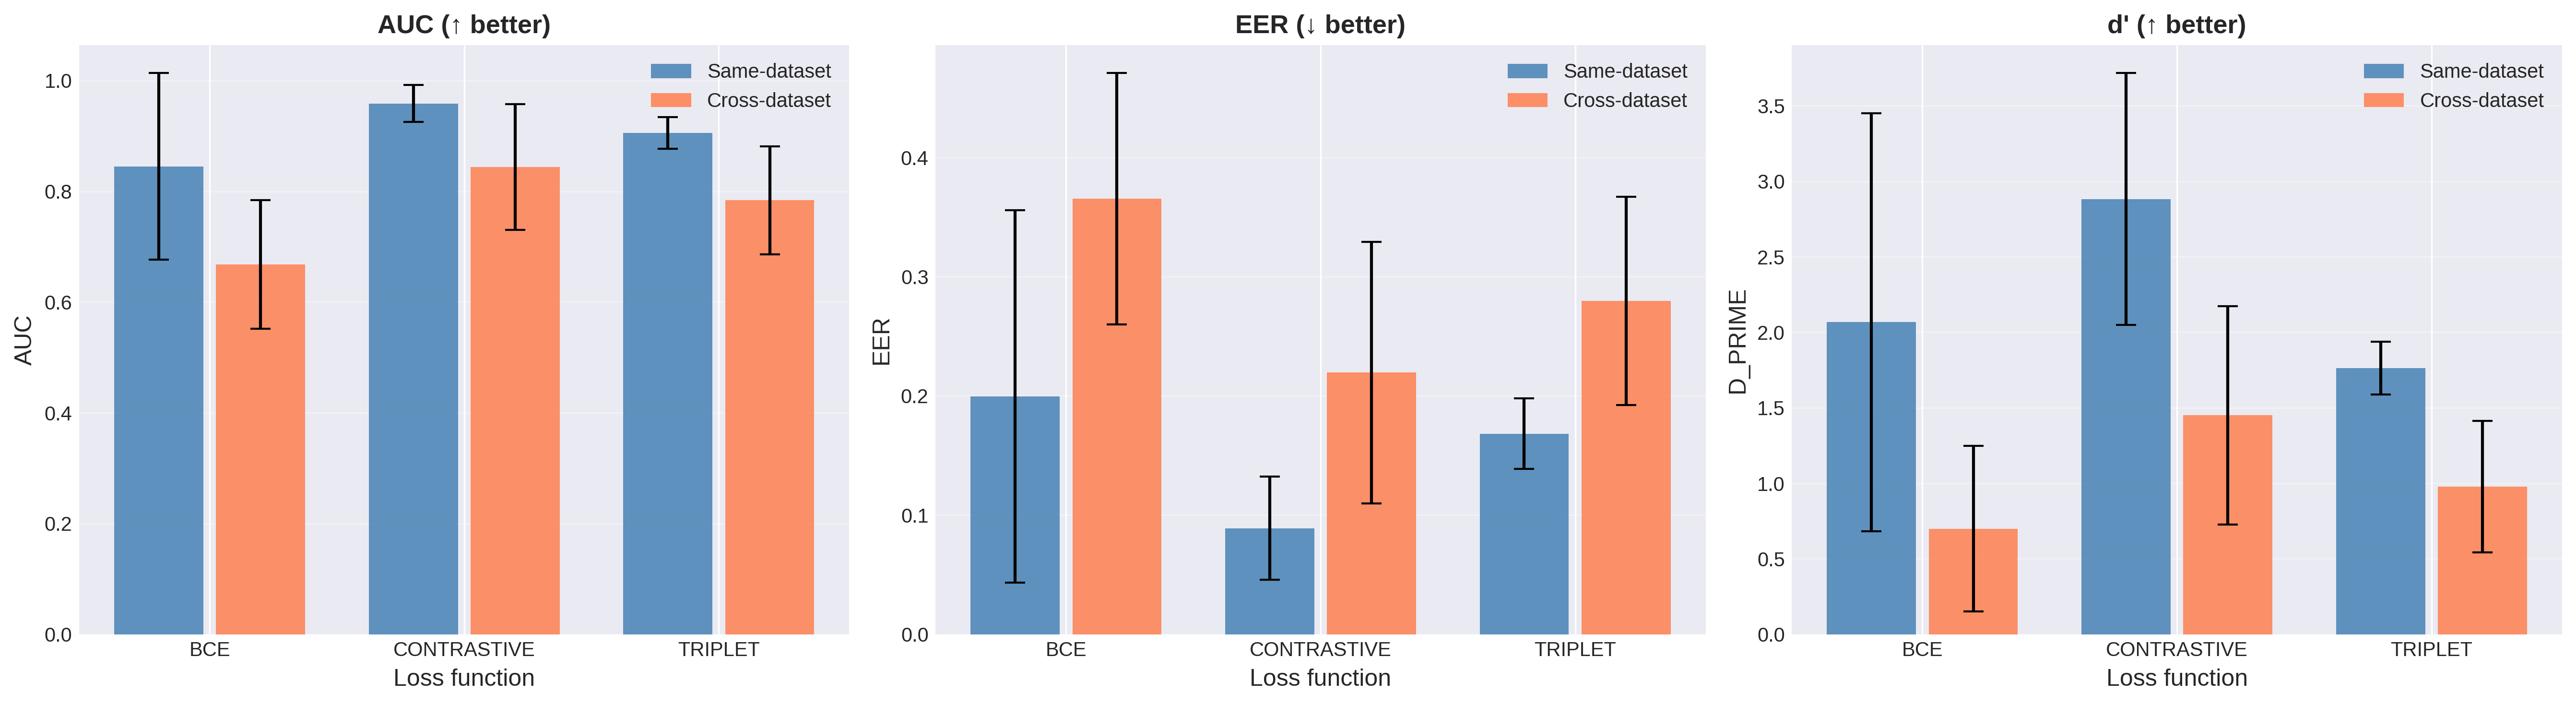
\includegraphics[width=\textwidth]{images/same_vs_cross_comparison_aggregated.png}
  \caption{AUC, EER and $d'$, same-dataset vs.\ cross-dataset,
  aggregated per loss (mean $\pm$ std across 6 backbones).}
  \label{fig:same-vs-cross}
\end{figure}

\subsection{Fixed operating points (FAR/FRR trade-off)}
\label{sec:operating-points}

Fixed operating points provide a complementary view of verification performance by quantifying the proportion of genuine pairs correctly accepted (GAR) under stringent false-acceptance constraints. In particular, FAR values of 1\% and 0.1\% represent increasingly conservative operating conditions, making the corresponding GAR values informative of how well a model maintains genuine-user acceptance while limiting false matches. The results also highlight the substantial impact of the dataset shift: while the best same-dataset configuration maintains relatively high GAR at both operating points, cross-dataset performance deteriorates markedly, especially at FAR$=0.1\%$. This indicates that a high overall discrimination capability does not necessarily translate into robust performance in low-FAR operating regimes, which are particularly relevant for practical biometric verification systems.

\begin{table}[htbp]
  \centering
  \caption{GAR at fixed FAR, best (backbone, loss) per split
  (Table~\ref{tab:ours-best}).}
  \label{tab:operating-points}
  \small
  \begin{tabular}{lcc}
    \toprule
    Split & GAR@FAR1\% & GAR@FAR0.1\% \\
    \midrule
    IAM$\to$IAM (MobileNetV3-Large, Contr.)     & 87.5\% & 72.4\% \\
    IAM$\to$RIMES (EfficientNet-B1, Contr.)     & 15.9\% & 4.6\%  \\
    RIMES$\to$IAM (EfficientNet-B0, Contr.)     & 62.6\% & 13.0\% \\
    RIMES$\to$RIMES (ResNet-18, Contr.)         & 53.9\% & 11.5\% \\
    \bottomrule
  \end{tabular}
\end{table}

EER can hide substantial performance differences at strict operating points. For example, the best same-dataset configuration achieves a GAR of 87.5\% at FAR $=1\%$ on IAM$\to$IAM, corresponding to a genuine rejection rate of 12.5\%. On RIMES$\to$RIMES, the GAR decreases from 53.9\% at FAR $=1\%$ to only 11.5\% at FAR $=0.1\%$, corresponding to genuine rejection rates of 46.1\% and 88.5\%, respectively. Cross-dataset performance is markedly worse, with GAR falling to the single-digit range at FAR $=0.1\%$ for IAM$\to$RIMES (4.6\%), corresponding to a genuine rejection rate of 95.4\%. These results illustrate that good overall discrimination, as reflected by EER, does not necessarily translate into effective operation under stringent false-acceptance constraints.

\subsection{Per-backbone analysis}
\label{sec:per-backbone}

\textbf{Collapsed models.} Four (backbone, loss, split) configurations
are collapsed (AUC $\approx$ chance), all under BCE:
\begin{itemize}
  \item MobileNetV3-Large / IAM$\to$RIMES: AUC $=0.528$
  \item MobileNetV3-Small / IAM$\to$RIMES: AUC $=0.516$
  \item MobileNetV3-Small / RIMES$\to$IAM: AUC $=0.540$
  \item EfficientNet-B1 / RIMES$\to$RIMES: AUC $=0.468$
\end{itemize}
This explains BCE's large across-backbone variance in
Sections~\ref{sec:same-dataset}--\ref{sec:cross-dataset}.

\textbf{Contrastive-over-BCE AUC gain}, averaged across all four
splits per backbone: MobileNetV3-Small ($+0.241$), EfficientNet-B1
($+0.190$), ResNet-34 ($+0.163$), EfficientNet-B0 ($+0.122$),
MobileNetV3-Large ($+0.093$), ResNet-18 ($+0.061$). ResNet-18 is the
only backbone with zero collapsed BCE configurations and benefits
least from switching losses.

\begin{figure}[htbp]
  \centering
  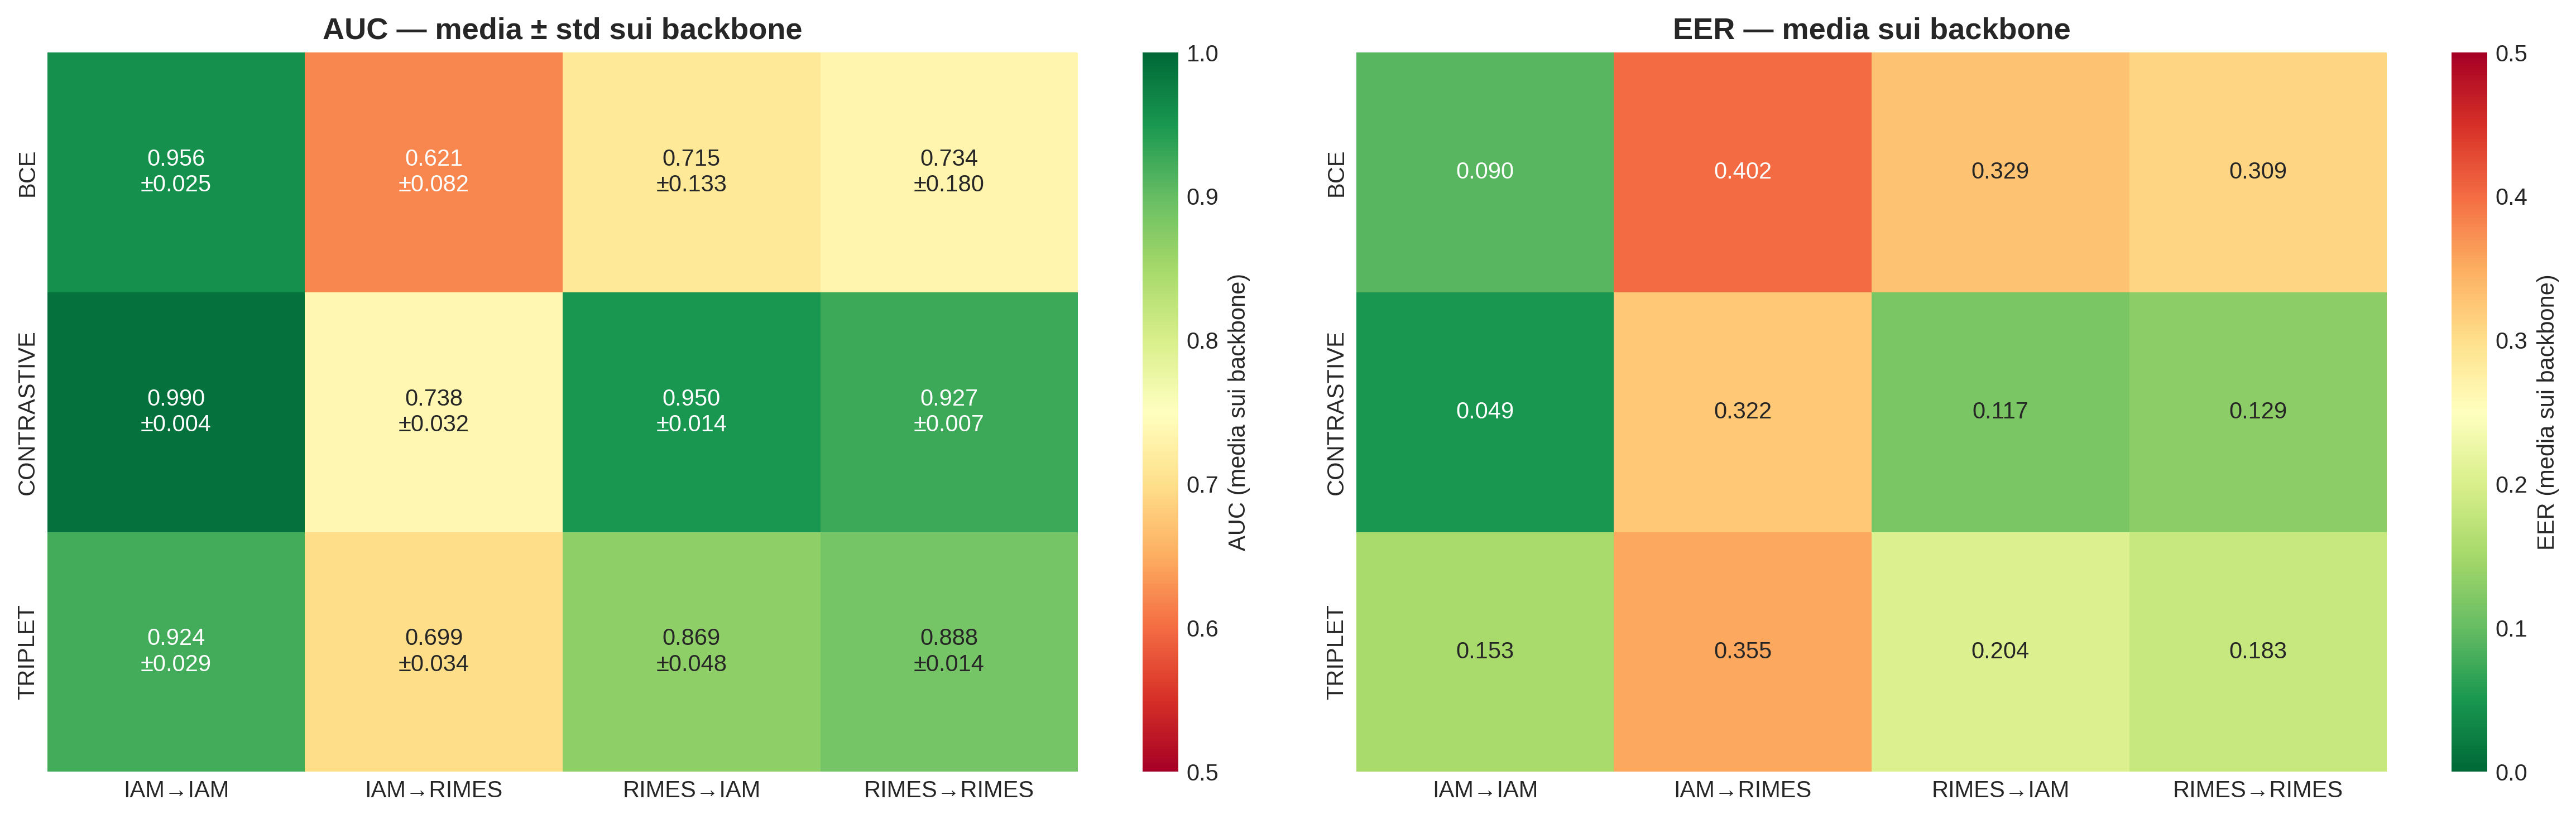
\includegraphics[width=\textwidth]{images/metrics_heatmap_aggregated.png}
  \caption{AUC and EER, mean across the 6 backbones, per
  loss$\times$split combination.}
  \label{fig:heatmap-aggregated}
\end{figure}

Figure~\ref{fig:heatmap-aggregated}: across-backbone AUC std is tight
under Contrastive throughout ($\pm0.004$--$\pm0.032$) but large under
BCE on the two splits with collapsed models (RIMES$\to$RIMES
$\pm0.180$, RIMES$\to$IAM $\pm0.133$). IAM$\to$RIMES is the hardest
cell under every loss (AUC $\leq0.738$); RIMES$\to$IAM under
Contrastive (AUC $0.950$) is close to same-dataset RIMES$\to$RIMES
($0.927$) despite being cross-dataset.

\textbf{Aggregate profile across all losses and splits.}

\begin{table}[htbp]
  \centering
  \caption{Per-backbone verification metrics, averaged across all 12
  loss$\times$split combinations.}
  \label{tab:radar-values}
  \small
  \begin{tabular}{lccccc}
    \toprule
    Backbone & AUC & EER (\%) & $d'$ & GAR@FAR1\% & GAR@FAR0.1\% \\
    \midrule
    ResNet-18            & \textbf{0.869} & \textbf{19.2} & \textbf{1.84} & 9.8\%  & 23.3\% \\
    EfficientNet-B0      & 0.849 & 20.2 & 1.75 & 10.0\% & 25.3\% \\
    EfficientNet-B1      & 0.838 & 21.1 & 1.77 & 14.3\% & \textbf{31.0\%} \\
    MobileNetV3-Large    & 0.833 & 22.3 & 1.59 & 13.1\% & 27.1\% \\
    ResNet-34            & 0.828 & 23.1 & 1.52 & 9.8\%  & 20.2\% \\
    MobileNetV3-Small    & 0.788 & 26.3 & 1.38 & \textbf{14.8\%} & 25.0\% \\
    \bottomrule
  \end{tabular}
\end{table}

\begin{figure}[htbp]
  \centering
  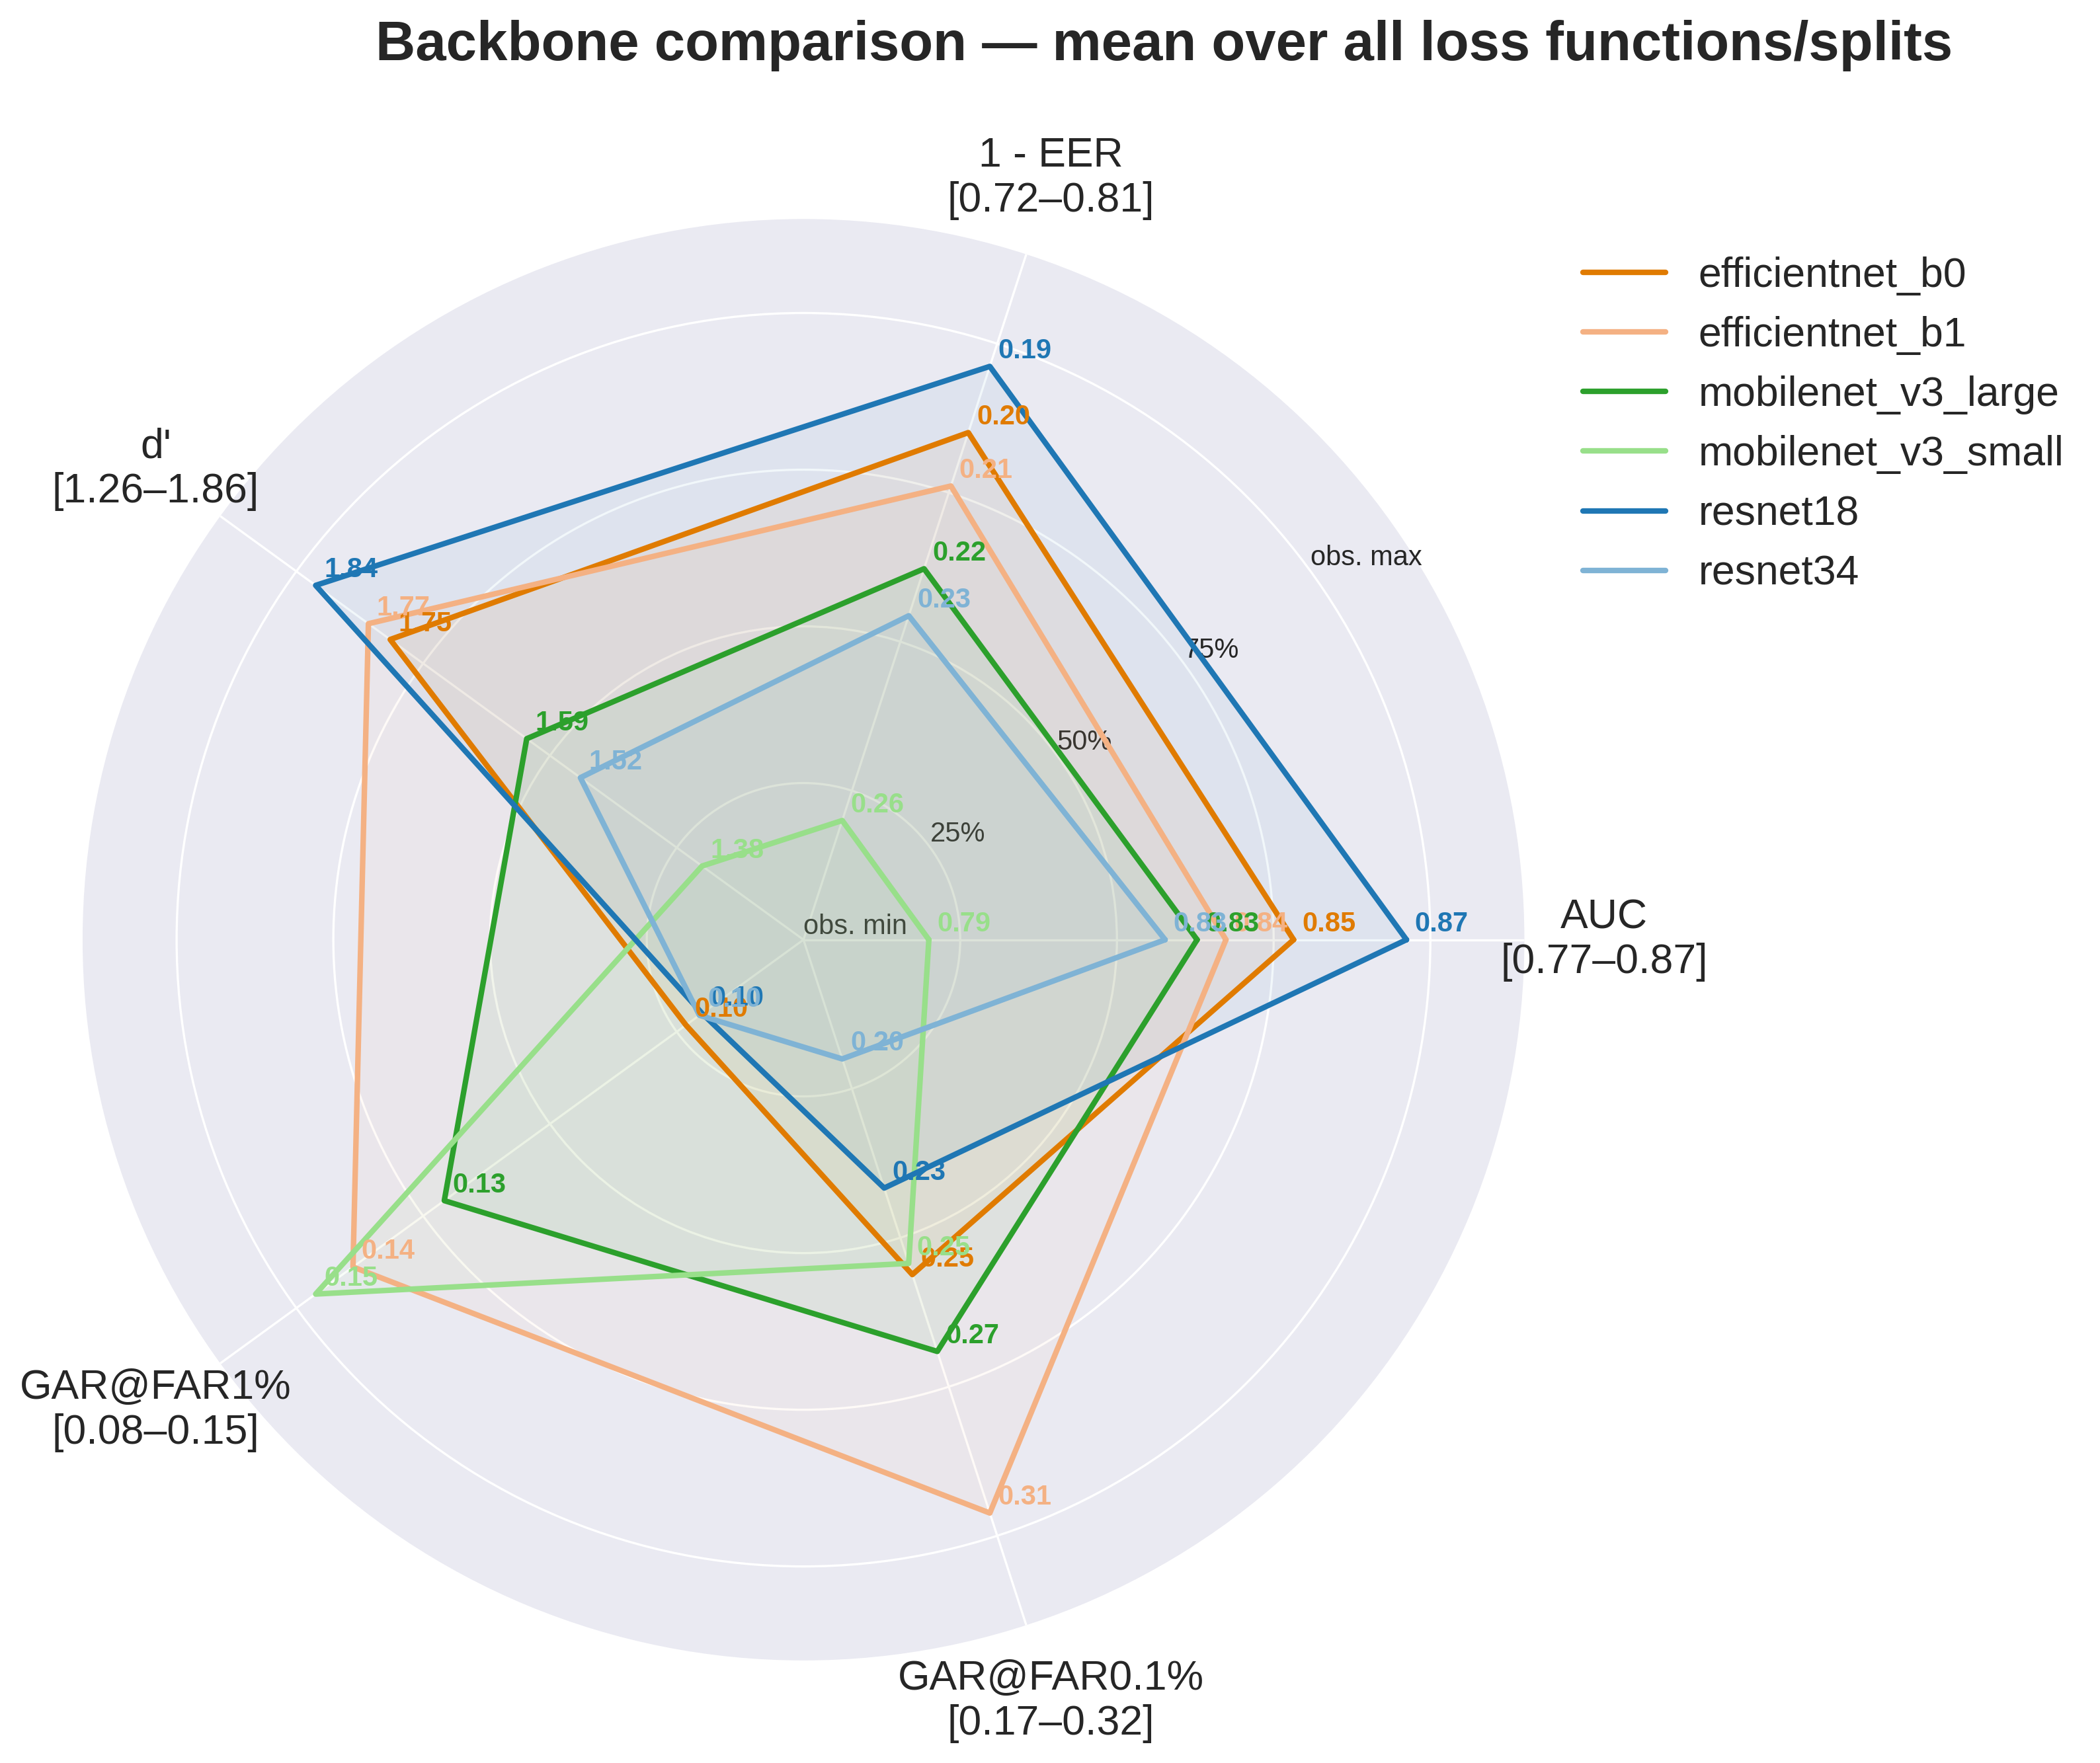
\includegraphics[width=0.75\textwidth]{images/radar_backbone_comparison.png}
  \caption{Per-backbone verification profile, averaged across all loss
  functions and dataset splits. Axis ranges scaled between observed
  min/max per metric; annotated values are raw means
  (Table~\ref{tab:radar-values}). Color by architecture family (blue:
  ResNet, orange: EfficientNet, green: MobileNetV3), darker shade =
  larger variant.}
  \label{fig:radar-backbone}
\end{figure}

ResNet-18 ranks first on AUC, EER and $d'$, but has the lowest
GAR@FAR1\% (9.8\%) and second-lowest GAR@FAR0.1\% (23.3\%) of all six
backbones. Overall separability and low-FAR-tail behavior are
therefore decoupled for this backbone: a small number of
high-scoring impostor pairs depresses GAR at strict thresholds without
affecting AUC/EER, consistent with the boundary-saturated impostor
tail reported for ResNet-18 under Contrastive on cross-dataset splits
(Section~\ref{sec:failure-analysis}).

EfficientNet-B1 shows the inverse profile: fourth on AUC, third on
EER/$d'$, but highest GAR@FAR0.1\% (31.0\%, $+7.7$ points over
ResNet-18).

MobileNetV3-Small has the worst AUC, EER and $d'$ of all six backbones,
consistent with its two collapsed BCE configurations, yet the highest
GAR@FAR1\% (14.8\%) — an isolated-threshold effect, not a
discriminability advantage.

Within the ResNet family, ResNet-34 underperforms ResNet-18 on every
metric except GAR@FAR1\% (near-tied, 9.8\% vs.\ 9.8\%), despite twice
the parameter count; no comparable inversion occurs between
EfficientNet-B0/B1. ResNet-34 is the only backbone that leads on no
metric in Table~\ref{tab:radar-values}.

Taken together, these results lead us to select ResNet-18 as the backbone for the subsequent analyses.


\subsection{Paired analysis of loss-function performance}
\label{sec:significance}

\begin{table}[htbp]
  \centering
  \caption{Paired Wilcoxon signed-rank test on AUC ($n=24$: 6 backbones
  $\times$ 4 splits).}
  \label{tab:wilcoxon}
  \begin{tabular}{lccccc}
    \toprule
    Comparison & Mean AUC (A) & Mean AUC (B) & $W$ & $p$ & Effect size \\
    \midrule
    BCE vs.\ Contrastive     & 0.756 & 0.901 & 1.0  & $2.38\times10^{-7}$ & $-0.993$ \\
    BCE vs.\ Triplet         & 0.756 & 0.845 & 63.0 & $0.0115$             & $-0.580$ \\
    Contrastive vs.\ Triplet & 0.901 & 0.845 & 0.0  & $1.19\times10^{-7}$ & $+1.000$ \\
    \bottomrule
  \end{tabular}
\end{table}

Because the 24 observations are not fully independent experimental replicates---they share the same backbone architectures, dataset splits, and underlying data, and each configuration is represented by a single training run---the Wilcoxon tests are interpreted as paired analyses of the consistency of loss-function differences across configurations, rather than as evidence from 24 independent training experiments. Under this interpretation, all three pairwise comparisons are statistically significant at $\alpha=0.05$. Contrastive significantly outperforms both BCE and Triplet, with very large effect sizes ($\rho=-0.993$ and $\rho=+1.000$, respectively; both $p<10^{-6}$). Triplet also outperforms BCE, although the effect is substantially smaller ($\rho=-0.580$, $p=0.0115$). Since the training recipes are uniform across losses (Section~\ref{subsubsec:dataset-pairings}), these differences are consistent with an effect of the loss objective itself. However, as discussed in Section~\ref{sec:per-backbone}, Contrastive's overall advantage does not necessarily reflect a uniform improvement across all architectures; part of its gain arises from its greater robustness on architectures for which BCE exhibits higher variability.

\subsection{High-precision validation with an exhaustive impostor pool}
\label{sec:exhaustive}

For ResNet-18 + Contrastive trained on RIMES and evaluated on the
\emph{full} IAM impostor pool (4{,}051 genuine pairs against
1{,}179{,}440 impostor pairs, $\sim\!291\times$ the balanced
protocol's impostor count), the exhaustive-pool re-evaluation gives:

\begin{table}[htbp]
  \centering
  \caption{Exhaustive-impostor-pool validation, RIMES$\to$IAM,
  ResNet-18 + Contrastive, vs.\ the balanced protocol.}
  \label{tab:exhaustive}
  \small
  \begin{tabular}{lcccc}
    \toprule
    Protocol & Impostor pairs & AUC & EER & GAR@1\% \\
    \midrule
    Balanced   & 4{,}051       & 0.967 & 8.2\%  & 62.6\% \\
    Exhaustive & 1{,}179{,}440 & 0.945 & 13.0\% & 34.5\% \\
    \bottomrule
  \end{tabular}
\end{table}

The exhaustive pool shows a genuine, non-trivial degradation relative
to the balanced protocol (AUC $0.967\to0.945$; EER $8.2\%\to13.0\%$;
GAR@1\% $62.6\%\to34.5\%$), indicating that 1:1 balanced impostor
subsampling in the main sweep was moderately optimistic for this
configuration. This is run for a single (backbone, loss, split) triple
only, given the cost of exhaustive scoring, and does not revisit the
per-backbone (Section~\ref{sec:per-backbone}) or Wilcoxon
(Section~\ref{sec:significance}) analyses.

\subsection{Best-model summary}
\label{sec:roc-det}

\begin{table}[htbp]
  \centering
  \caption{Best-performing (backbone, loss) configuration per split
  (Table~4).}
  \label{tab:ours-best}
  \small
  \begin{tabular}{llcc}
    \toprule
    Split & Best (backbone, loss) & AUC & EER \\
    \midrule
    IAM$\to$IAM     & MobileNetV3-Large, Contrastive & 0.995 & 3.1\%  \\
    IAM$\to$RIMES   & EfficientNet-B1, Contrastive   & 0.772 & 29.6\% \\
    RIMES$\to$IAM   & EfficientNet-B0, Contrastive   & 0.967 & 8.2\%  \\
    RIMES$\to$RIMES & ResNet-18, Contrastive         & 0.934 & 11.5\% \\
    \bottomrule
  \end{tabular}
\end{table}

\begin{table}[htbp]
  \centering
  \caption{Classification metrics at the EER threshold, best
  (backbone, loss) per split (Table~4).}
  \label{tab:classification-metrics}
  \small
  \begin{tabular}{lcccccc}
    \toprule
    Split & Accuracy & Precision & Recall & F1 & $\mu_g/\mu_i$ & $\sigma_g/\sigma_i$ \\
    \midrule
    IAM$\to$IAM     & 0.969 & 0.969 & 0.969 & 0.969 & 0.893/0.005 & 0.118/0.277 \\
    IAM$\to$RIMES   & 0.704 & 0.704 & 0.704 & 0.704 & 0.829/0.648 & 0.170/0.219 \\
    RIMES$\to$IAM   & 0.918 & 0.918 & 0.918 & 0.918 & 0.938/0.413 & 0.110/0.294 \\
    RIMES$\to$RIMES & 0.885 & 0.885 & 0.885 & 0.885 & 0.791/0.063 & 0.284/0.357 \\
    \bottomrule
  \end{tabular}
\end{table}

As noted in Section~\ref{sec:protocol}, these figures are computed at
the EER threshold of each model on its own evaluation set, not an
independently calibrated threshold. The provided ROC/DET/distribution
figures (Figures~\ref{fig:roc}--\ref{fig:distributions}) cover
ResNet-18 across all 12 loss$\times$split combinations, and are shown
as a representative supplementary panel rather than as the
aggregate-best-per-split configurations of
Table~\ref{tab:ours-best} (which include MobileNetV3-Large and
EfficientNet-B0/B1 for three of the four splits).

\begin{figure}[htbp]
  \centering
  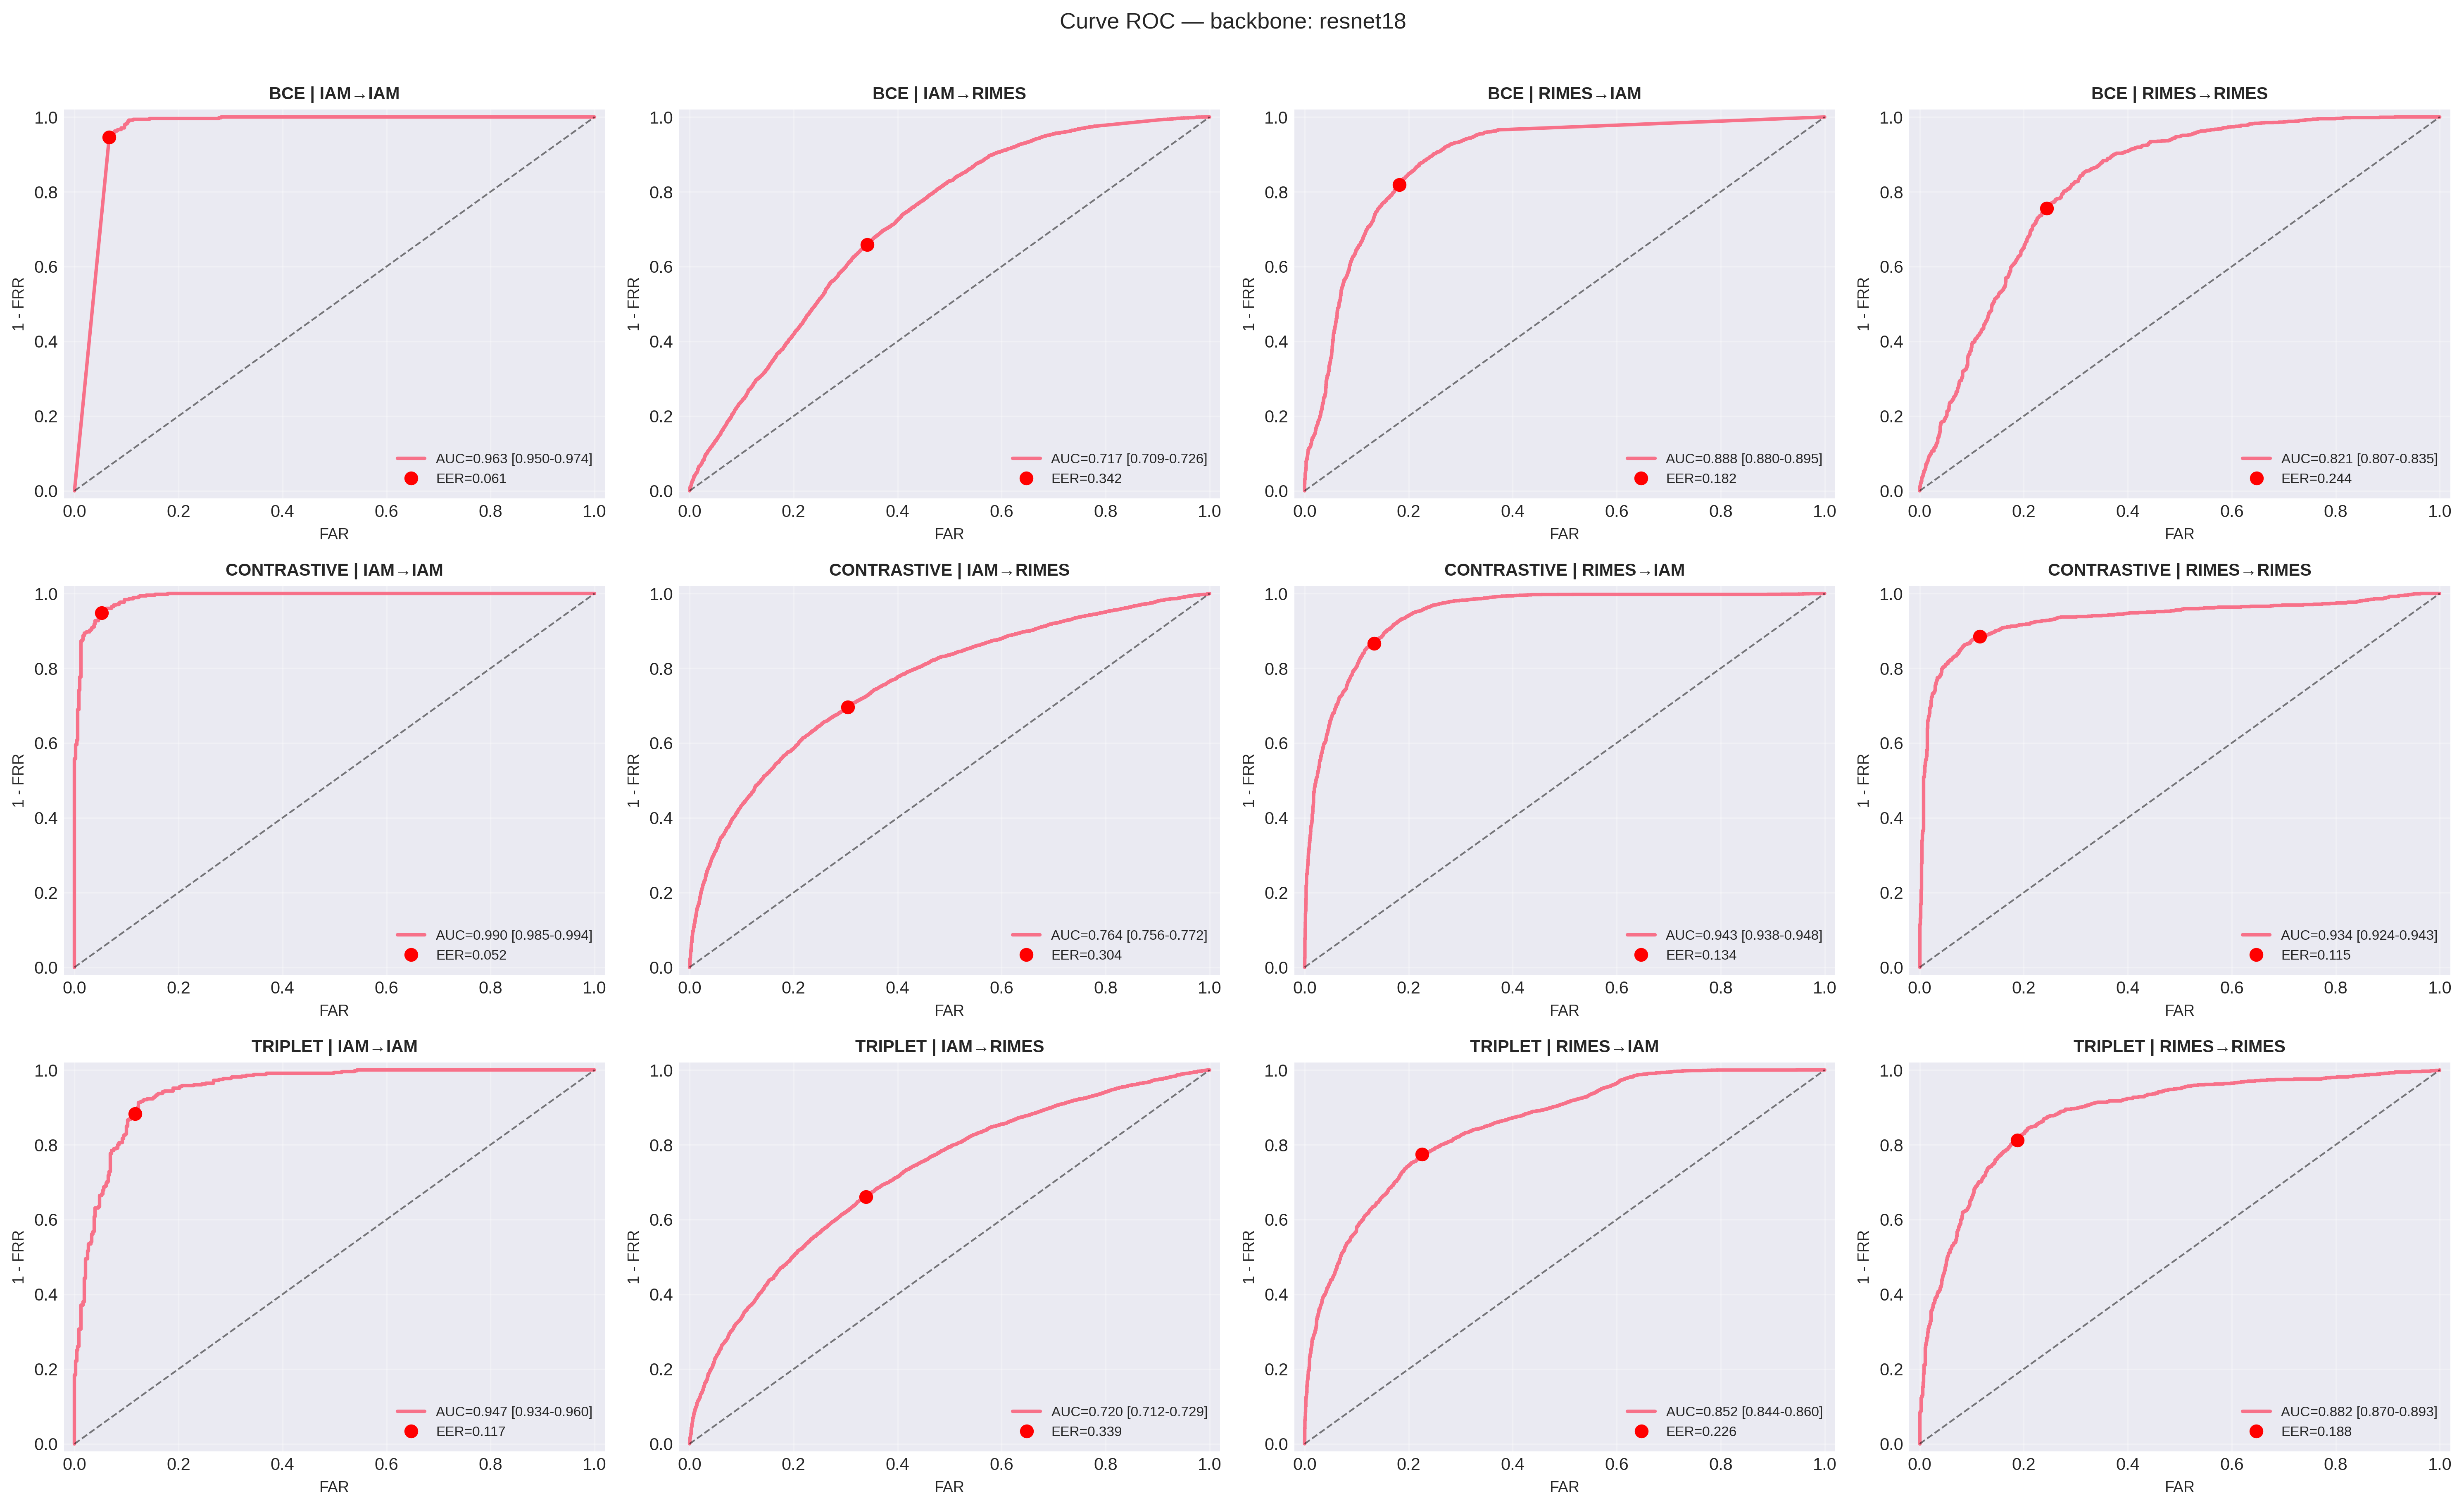
\includegraphics[width=\textwidth]{images/roc_curves_resnet18.png}
  \caption{ROC curves, ResNet-18, all losses/splits.
  Bootstrap 95\% confidence intervals for AUC are reported in each
  panel legend.}
  \label{fig:roc}
\end{figure}

The ROC curves in Figure~\ref{fig:roc} report bootstrap 95\%
confidence intervals alongside each AUC estimate. Contrastive
achieves the highest AUC on all four splits for ResNet-18 (IAM$\to$IAM:
0.990; IAM$\to$RIMES: 0.764; RIMES$\to$IAM: 0.943; RIMES$\to$RIMES:
0.934), consistently outperforming BCE and Triplet across the full
FAR range rather than only near the EER operating point. The ordering
of BCE and Triplet is not fixed across splits: BCE outperforms Triplet
on two of the four splits (IAM$\to$IAM, RIMES$\to$IAM,), but Triplet marginally exceeds BCE on IAM$\to$RIMES, the hardest cross-dataset pairing for this
backbone, and RIMES$\to$RIMES. Confidence-interval width is governed primarily by
evaluation-set size rather than by the same-vs-cross-dataset
distinction: the narrowest interval overall belongs to
Contrastive/IAM$\to$IAM (width $0.009$, $n=958$ pairs), while
BCE/IAM$\to$IAM and BCE/RIMES$\to$RIMES -- despite being a same-dataset split -- shows the widest intervals (width $0.024$ and $0.028$, respectively), reflecting their comparatively
small test sets relative to the cross-dataset splits (e.g.\
IAM$\to$RIMES, $n=12{,}858$ pairs, CI width $0.016$--$0.017$ across
losses). At the shape level, the same-dataset curves (IAM$\to$IAM,
RIMES$\to$RIMES) rise sharply toward the top-left corner across all
three losses, whereas the cross-dataset curves -- particularly
IAM$\to$RIMES -- remain comparatively close to the chance diagonal
over a wide FAR range, visually corroborating the same-vs-cross-dataset
generalization gap discussed in Section~\ref{sec:cross-dataset}.

\begin{figure}[htbp]
  \centering
  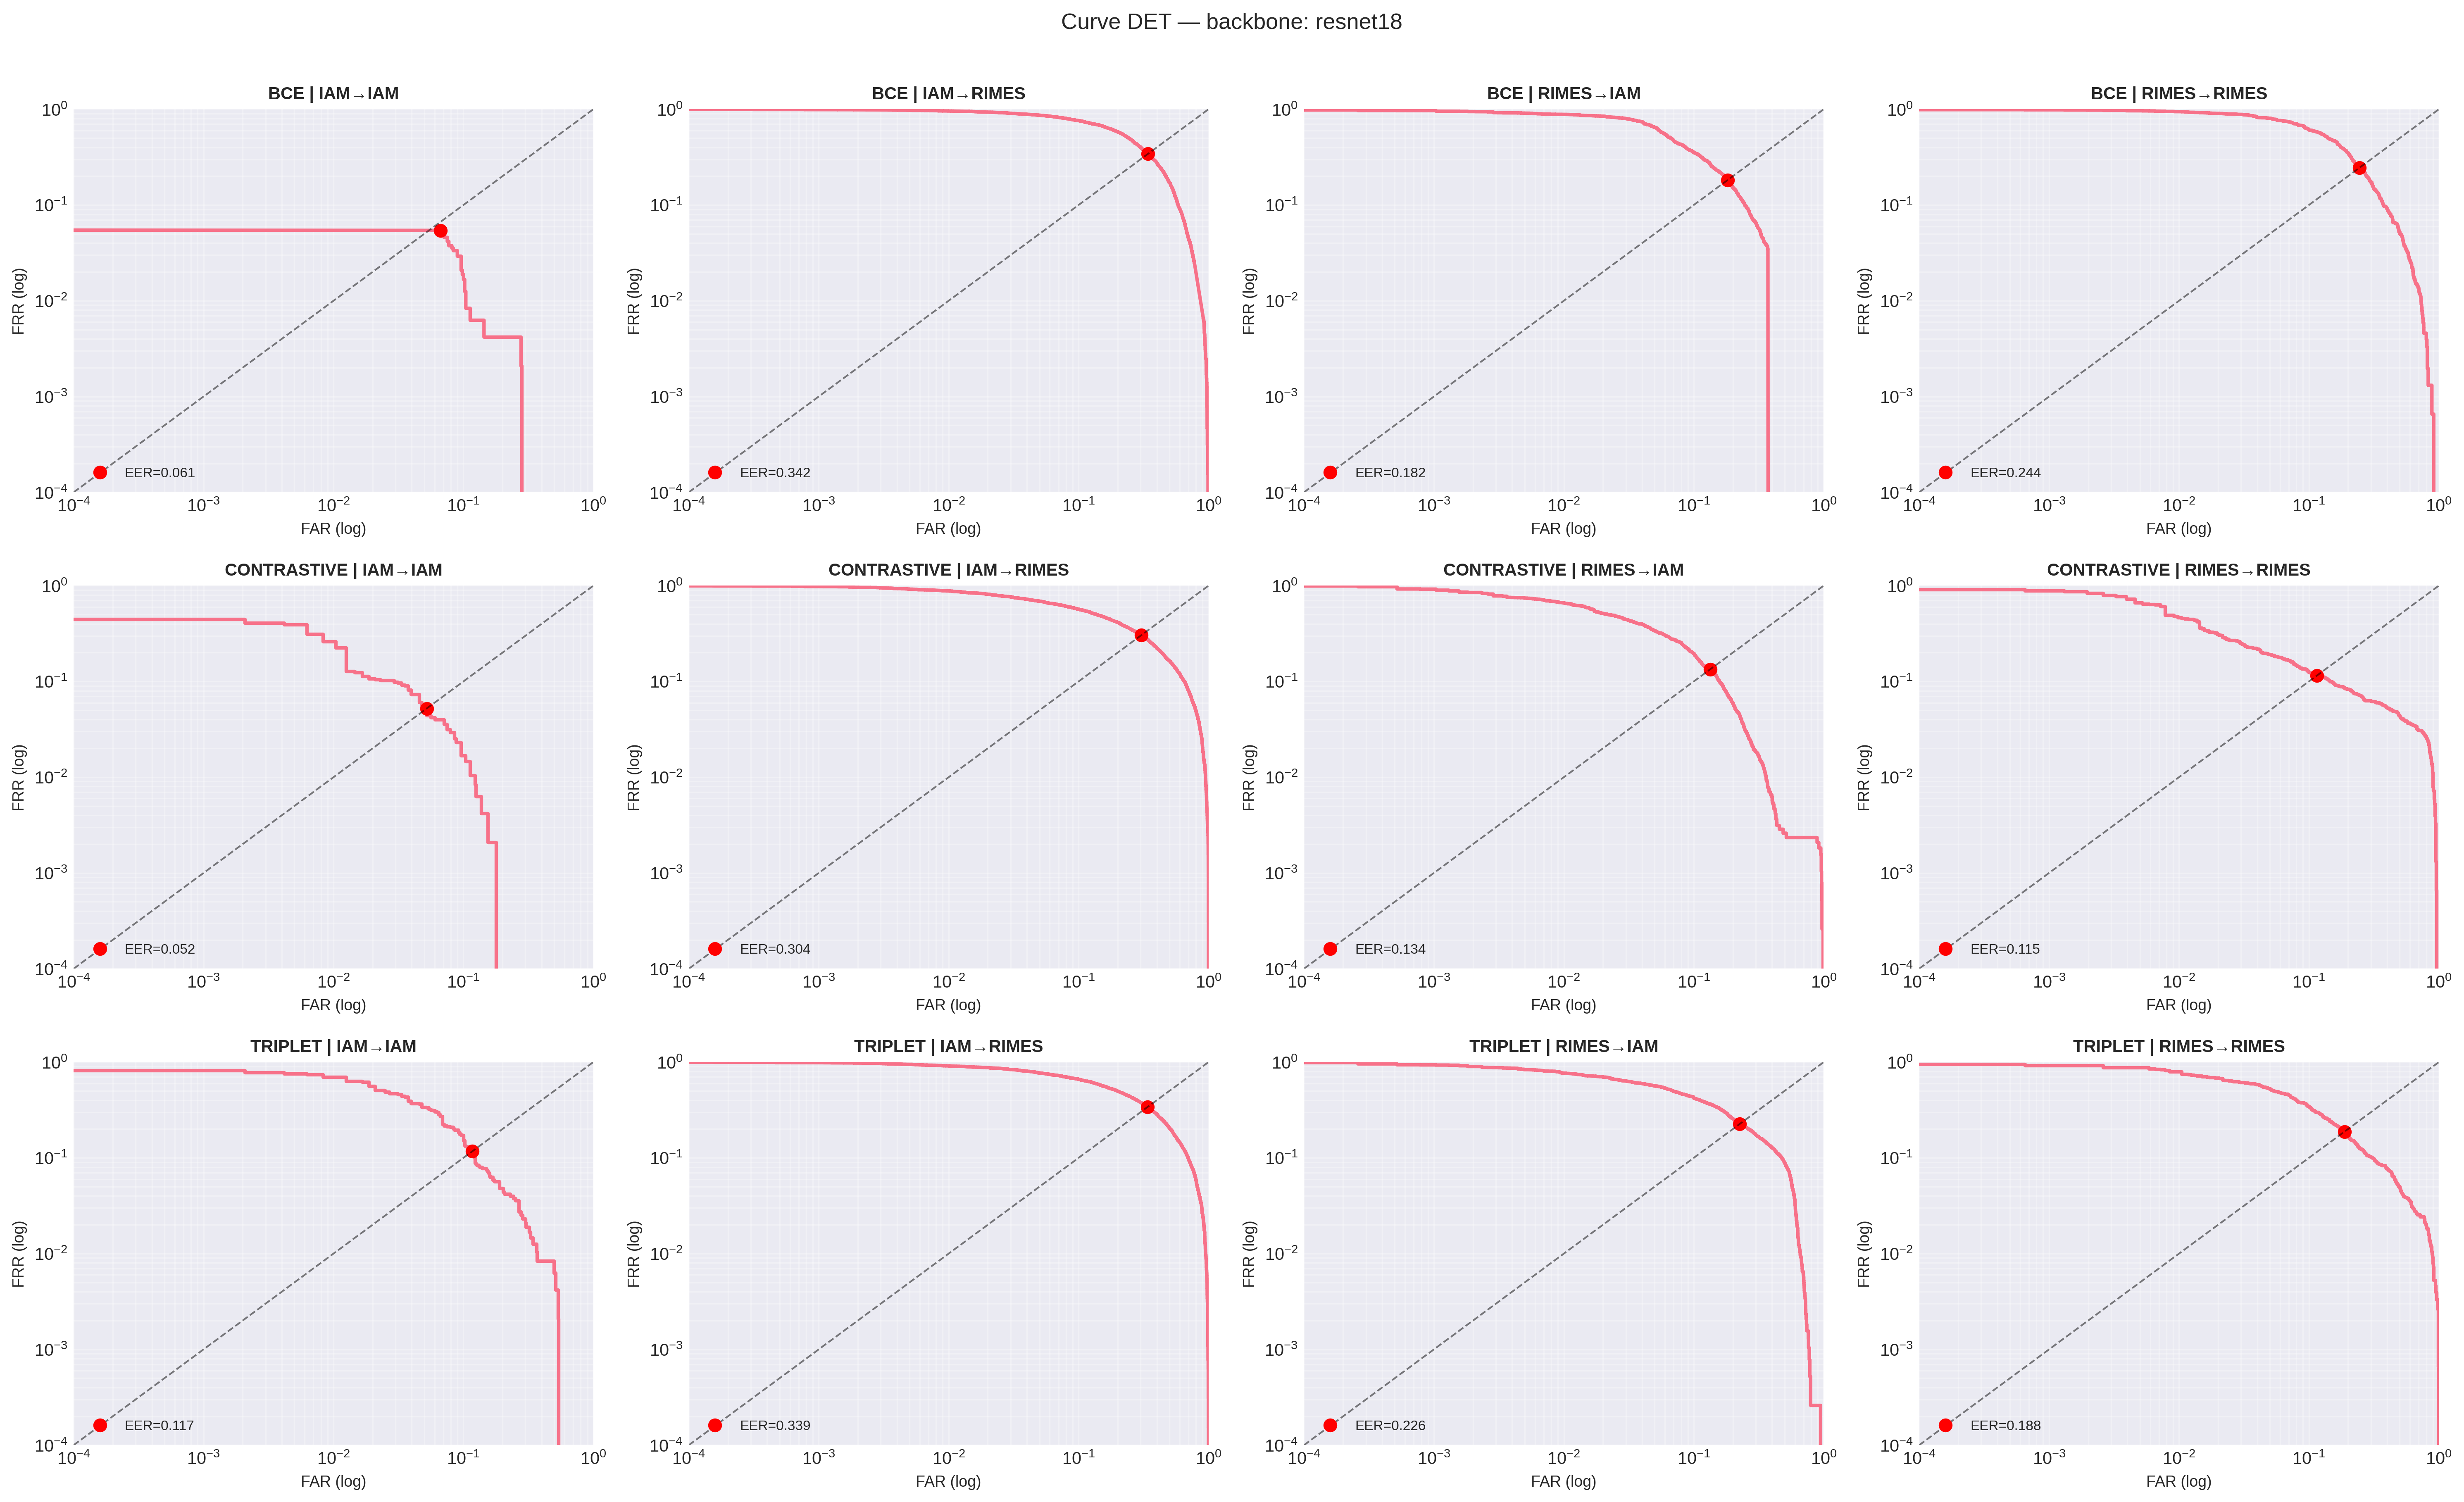
\includegraphics[width=\textwidth]{images/det_curves_resnet18.png}
  \caption{DET curves (log-log), ResNet-18, all losses/splits
  (supplementary).}
  \label{fig:det}
\end{figure}

The DET curves in Figure~\ref{fig:det} provide a visual representation
of the strong variation in verification performance across losses and
dataset splits. The IAM$\to$IAM curves are consistently the most
favorable, reaching relatively low FRR at small FAR values across all
three losses. However, the shape differs by loss: BCE exhibits a
pronounced, nearly flat plateau in the low-FAR region before dropping
sharply, Contrastive shows a comparable but noisier and less
perfectly flat shelf at a higher FRR level, while Triplet decreases
more smoothly and monotonically without a distinct plateau. In
contrast, the IAM$\to$RIMES curves remain close to the upper part of
the plot over a large portion of the FAR range for all three losses,
indicating a substantial loss of discrimination under the
cross-dataset shift, with a sharp drop only near each curve's EER
point. RIMES$\to$IAM shows intermediate behavior between the two
same-dataset splits and IAM$\to$RIMES, with Contrastive (EER $=13.4\%$)
clearly outperforming BCE (EER $=18.2\%$) and Triplet (EER $=22.6\%$).
The RIMES$\to$RIMES curves, evaluated on the second same-dataset
split, also show substantial variation across losses, with Contrastive
producing the most favorable operating characteristics and the lowest
EER ($11.5\%$ vs.\ $24.4\%$ for BCE and $18.8\%$ for Triplet). Overall,
the DET plots corroborate the strong dependence of verification
performance on the dataset pairing: the cross-dataset shift is
particularly detrimental for IAM$\to$RIMES, where all three losses
exhibit substantially higher FRR across the operating range than in
either same-dataset setting. Among the two cross-dataset splits,
Contrastive provides the more favorable behavior on RIMES$\to$IAM,
although its performance still degrades markedly relative to its own
same-dataset results under the IAM$\to$RIMES shift.

\subsection{Score distributions and the Gaussianity assumption}
\label{sec:distributions}

Shapiro--Wilk tests on all 72 genuine and 72 impostor score
distributions reject normality universally at $\alpha=0.05$ (largest
observed $p$-value $\sim2\times10^{-6}$, ResNet-18/Contrastive/RIMES$\to$RIMES
genuine scores); no distribution in the sweep is Gaussian-compatible.
Consequently, $d'$/decidability are reported throughout this paper
strictly as descriptive, rank-consistent indices rather than as
parametric inferential statistics.

\begin{figure}[htbp]
  \centering
  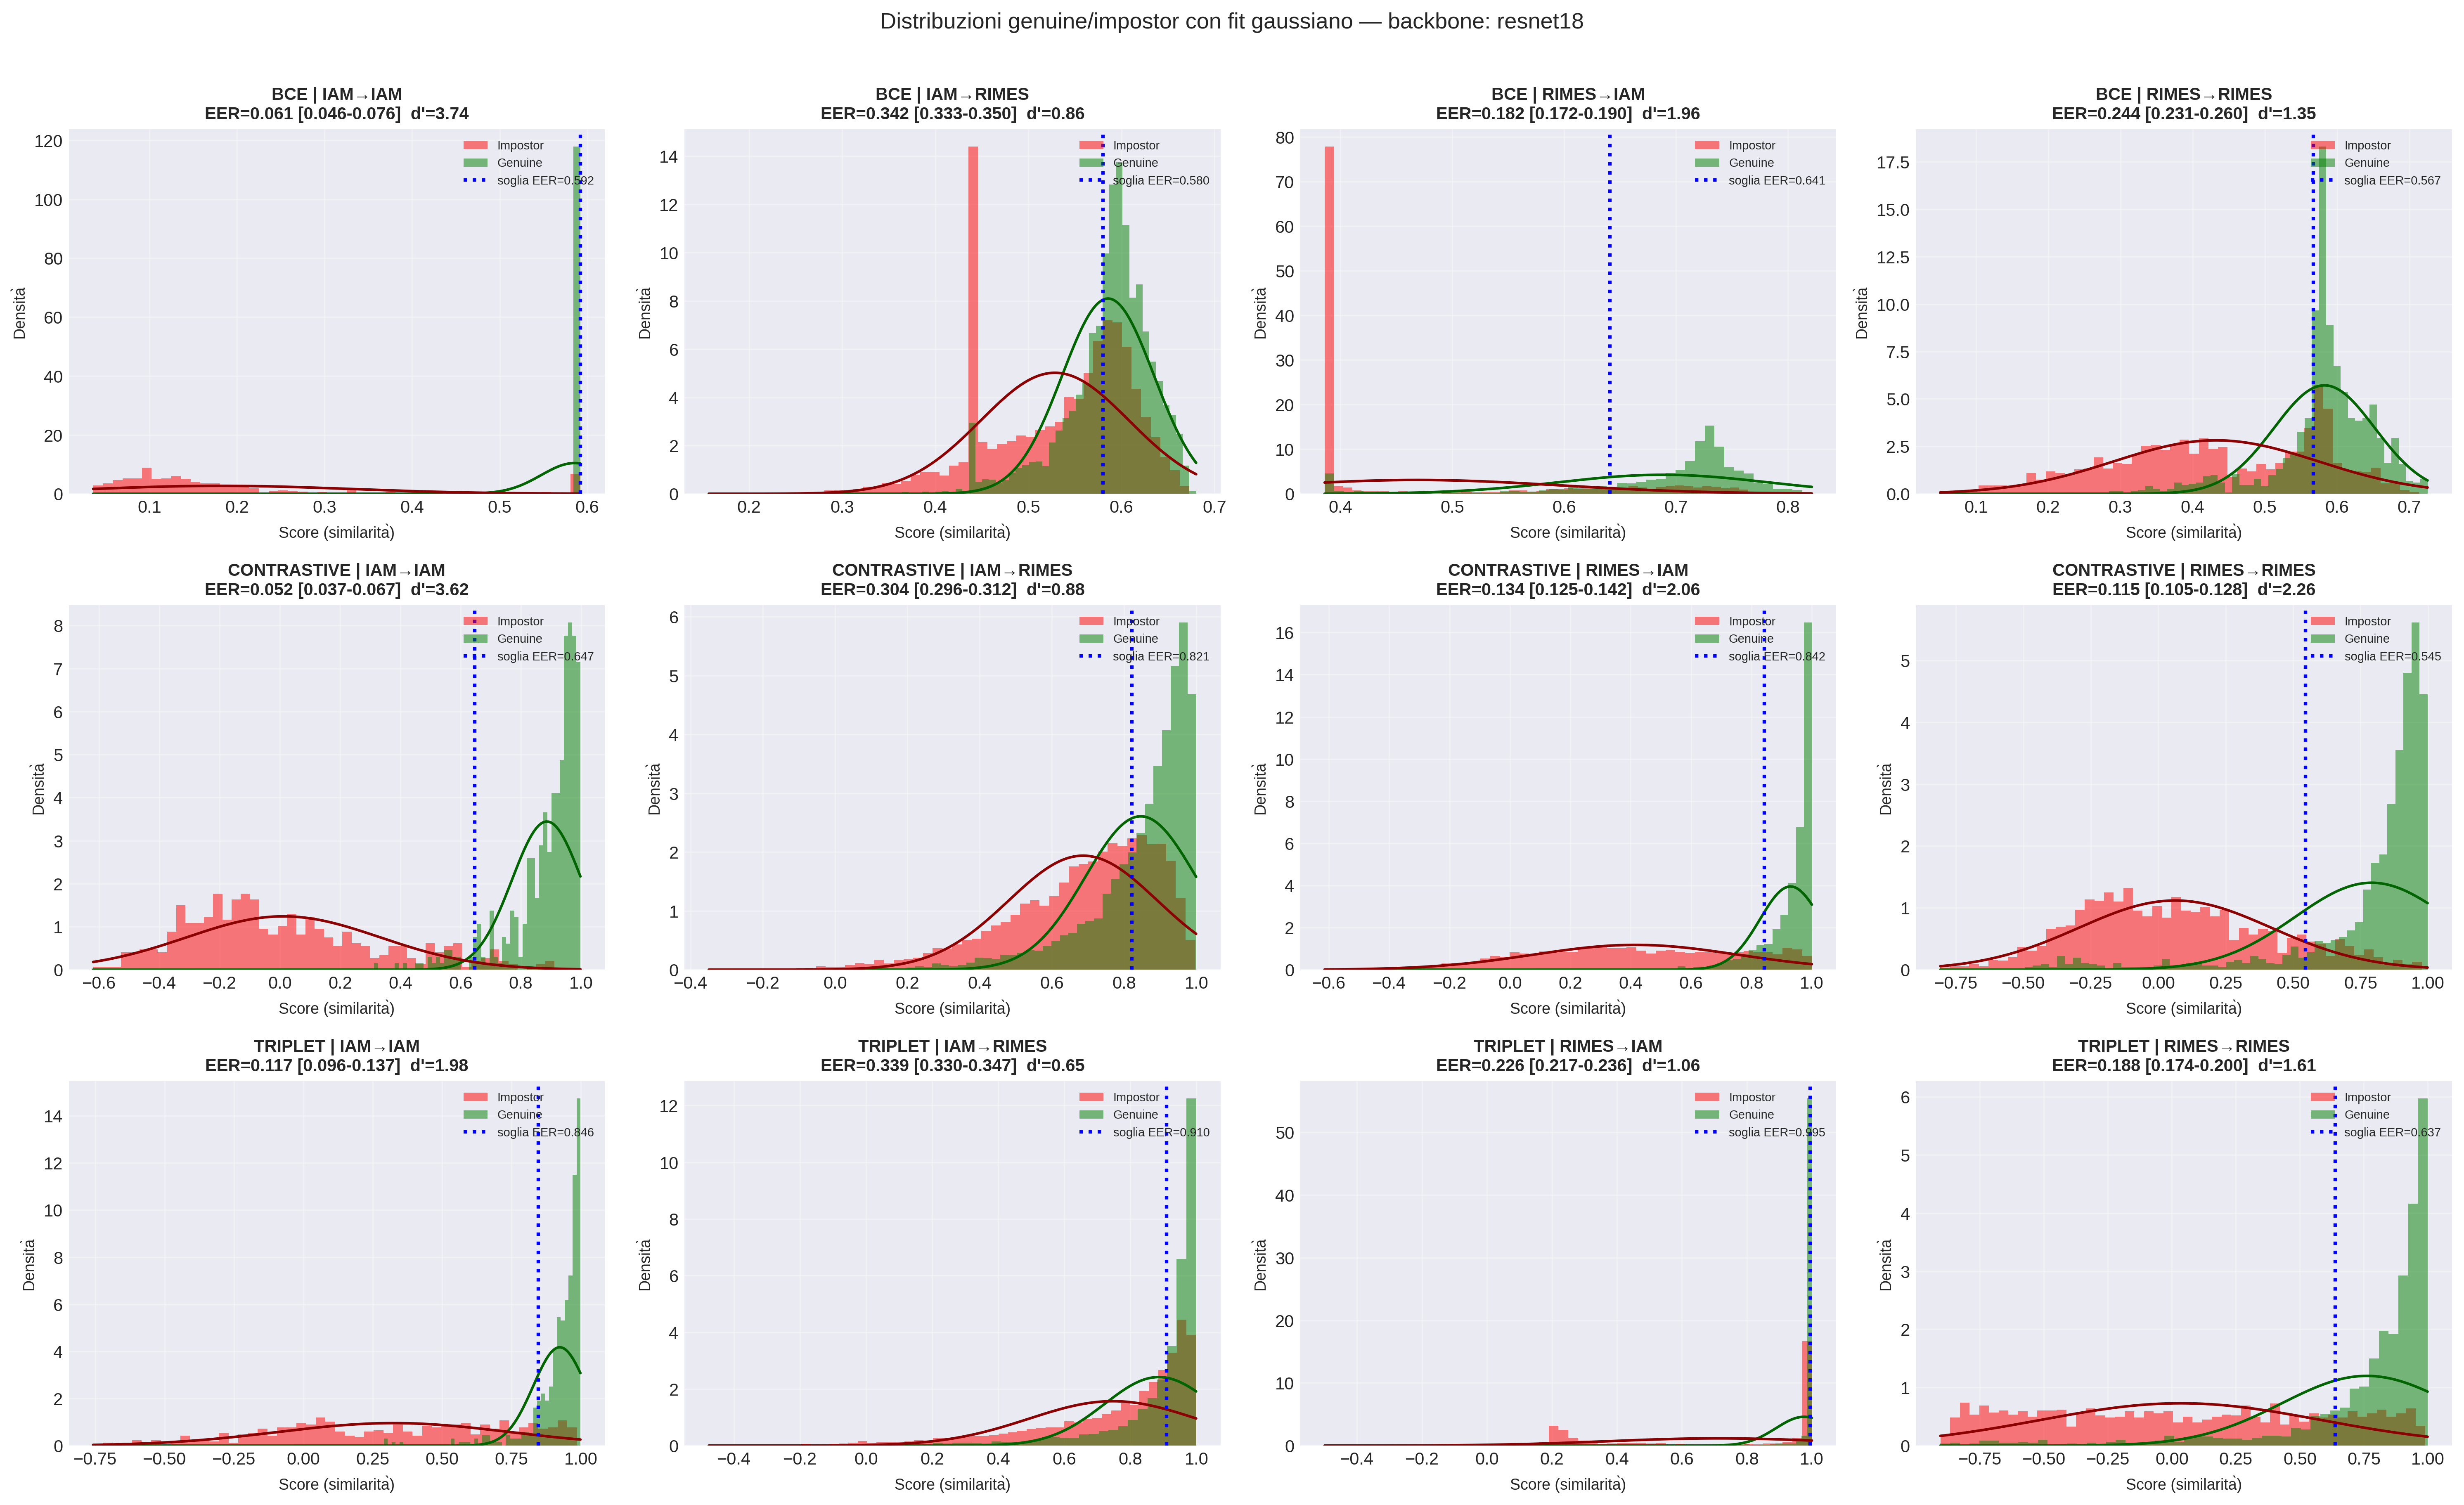
\includegraphics[width=\textwidth]{images/score_distributions_resnet18.png}
  \caption{Genuine (green)/impostor (red) scores with fitted Gaussian
  overlays, ResNet-18, all loss$\times$split combinations. Dotted
  lines: EER threshold. None of the 12 distributions shown pass
  Shapiro--Wilk at $\alpha=0.05$.}
  \label{fig:distributions}
\end{figure}

Visual inspection of Figure~\ref{fig:distributions} shows that
BCE/RIMES$\to$IAM and BCE/RIMES$\to$RIMES exhibit substantially more
genuine-impostor overlap than the same-dataset IAM$\to$IAM panel,
consistent with their comparatively higher EER ($18.2\%$ and $24.4\%$,
respectively, vs.\ $6.1\%$ for BCE/IAM$\to$IAM); this reflects a
genuine loss of separability under BCE on these splits, though for
ResNet-18 both configurations remain well above chance-level
discrimination (AUC $=0.888$ and $0.821$; ResNet-18 does not exhibit
any of the fully collapsed, near-chance BCE configurations documented
for other backbones in Section~\ref{sec:per-backbone}). Contrastive
and Triplet distributions, by contrast, display visible
boundary-clustered mass near the similarity limits $\pm 1$,
particularly for RIMES$\to$IAM.

A further pattern visible in Figure~\ref{fig:distributions} is that
under BCE, several impostor distributions exhibit a narrow, isolated
spike at a fixed low score (e.g.\ BCE/RIMES$\to$IAM, impostor mass
concentrated near score $\approx 0.39$; BCE/IAM$\to$RIMES, near
$\approx 0.44$), rather than a smooth unimodal shape -- a possible
signature of a degenerate embedding direction rather than genuine
score variability. Under Contrastive and Triplet, by contrast,
impostor distributions are broad and (generally) left-skewed while genuine
distributions are (gnerally) right-skewed and compressed near the similarity
ceiling ($\approx 1.0$), producing the asymmetric overlap responsible
for the boundary-saturation effect noted above; this asymmetry is most
pronounced for cross-dataset splits, and least pronounced for same-dataset splits,
mirroring the EER ordering across splits
(Tables~\ref{tab:same-dataset}--\ref{tab:cross-dataset}).

\subsection{Failure-case analysis}
\label{sec:failure-analysis}

We inspect failure modes of the strongest configuration per split
(Table~\ref{tab:ours-best}) using the ResNet-18 distribution plots
(Figure~\ref{fig:distributions}) and, for RIMES$\to$IAM (ResNet-18 +
Contrastive), a pair-level export of the top false accepts and false
rejects.

\begin{itemize}
\item\textbf{Distribution-level patterns.} Two failure modes are visible
for ResNet-18. First, BCE/IAM$\to$RIMES shows genuine and impostor
modes heavily overlapping around the same $0.5$--$0.6$ score region
(EER $=34.2\%$, $d'=0.86$), the weakest separation among all four
BCE panels and the closest ResNet-18 comes to the near-chance behavior
of the fully collapsed models in Section~\ref{sec:per-backbone} (none
of which involve ResNet-18); BCE/RIMES$\to$RIMES shows a milder
version, with a broader impostor distribution encroaching on the
genuine mode's lower tail (EER $=24.4\%$, $d'=1.35$) while the genuine
peak stays distinct. Second, under Contrastive on both cross-dataset
splits, a non-trivial fraction of impostor pairs saturate near the
maximum cosine similarity ($\approx1.0$), overlapping the genuine
mode; this produces the long, shallow DET tail in
Figure~\ref{fig:det} and explains why GAR at strict FAR
(Section~\ref{sec:operating-points}) collapses to single digits on
IAM$\to$RIMES despite a moderate mean EER ($32.2\%$).

\item \textbf{Pair-level inspection (RIMES$\to$IAM, ResNet-18 +
Contrastive).} Figure~\ref{fig:false-accepts} shows the top false
accepts (scores $0.9986$/$0.9964$, $\Delta \approx+0.155$/$+0.154$
above the $0.8424$ threshold): different writers sharing slant,
spacing, and regularity -- confident errors driven by surface
stylistic similarity the embedding does not disentangle from
identity, consistent with the boundary-saturation pattern above.
Figure~\ref{fig:false-rejects} shows the top false rejects (scores
$-0.3076$/$-0.2111$, $\Delta \approx-1.150$/$-1.054$ below threshold):
the \emph{same} writer across samples differing markedly in letter
size, stroke pressure, and legibility.
\end{itemize}

\begin{figure}[htbp]
  \centering
  
\includegraphics[width=0.9\linewidth]{images/resnet18_contrastive_rimes_to_iam_false_accepts_grid.png}
  \caption{Top false accepts, RIMES$\to$IAM, ResNet-18 + Contrastive.
  Each row shows one impostor pair scored well above the EER threshold
  ($0.8424$), with the assigned score and the margin $\Delta$ above
  threshold.}
  \label{fig:false-accepts}
\end{figure}

\begin{figure}[htbp]
  \centering
  
\includegraphics[width=0.9\linewidth]{images/resnet18_contrastive_rimes_to_iam_false_rejects_grid.png}
  \caption{Top false rejects, RIMES$\to$IAM, ResNet-18 + Contrastive.
  Each row shows one genuine pair scored well below the EER threshold
  ($0.8424$), with the assigned score and the margin $\Delta$ below
  threshold.}
  \label{fig:false-rejects}
\end{figure}

This intra-writer inconsistency is not an IAM artifact specific to
these two pairs: writer-to-sample counts in IAM are highly uneven (as
few as one page for roughly half of the 657 writers, up to 59 for a
single writer, see Subsection \ref{subsec:dataset-stats}), so writer identity does not
guarantee within-writer homogeneity of content, layout, or scale.
More fundamentally, forensic document-examination literature documents
\emph{multi-individuality of handwriting}\cite{MOSZCZYNSKI2019e4}: some writers maintain two
or more distinct styles used spontaneously or deliberately, which can
appear as different as two different people's handwriting to an
automated system trained on surface stylistic cues. This offers a mechanistic explanation for the
Contrastive-over-BCE cross-dataset gap
(Sections~\ref{sec:cross-dataset},~\ref{sec:significance}): a
representation invariant to stroke width, slant and spacing --
properties BCE's un-margined objective has less incentive to
suppress -- would better separate genuine pairs whose surface style
varies while remaining sensitive to the subtler, writer-specific
features (letter formation, proportions) that persist across such
variation. Under this reading, false rejects and false accepts have
distinct sources: the former is largely intra-writer style
variability inherent to IAM's uncontrolled-form collection protocol,
the latter is embedding under-disentanglement of surface style from
identity, and only the second is directly actionable via representation
learning.

High intra-writer variability can contribute to both types of verification errors. Genuine pairs may be falsely rejected when stylistic differences make samples from the same writer appear dissimilar. Conversely, impostor pairs may be falsely accepted when superficial similarities make different writers appear similar. This latter error can arise indirectly from the model learning to associate substantially different writing styles with the same writer during training: by observing diverse samples from the same writer, the model is encouraged to map stylistically different instances to similar representations, but this may also reduce its ability to distinguish writers who share similar surface styles.

This inspection covers a single (backbone, loss, split) triple and
the top-2 errors per failure mode; a systematic pair-level analysis
across the full test set, and a check of whether errors concentrate on
low-sample-count writers, is left to future work
(Section~\ref{sec:limitations}).

\subsection{Comparison with prior work}
\label{sec:sota}

Direct comparison is limited: most prior CNN-based work on IAM/RIMES
addresses closed-set \emph{identification} (top-1/mAP), not the
open-set, pairwise \emph{verification} protocol (EER/AUC) used here;
and methodologically comparable Siamese-verification studies are
evaluated on different scripts (Arabic/Chinese/Japanese), not
IAM/RIMES. With this caveat, Table~\ref{tab:sota} situates our EER
range within the broader literature rather than claiming a leaderboard
rank.

\begin{table}[htbp]
  \centering
  \caption{Prior work on CNN-based writer identification/verification.}
  \label{tab:sota}
  \small
  \begin{tabular}{lllll}
    \toprule
    Method & Task & Dataset & Metric & Value \\
    \midrule
    Fiel \& Sablatnig~\cite{fiel2015} & Identification (closed-set) & IAM (train), ICDAR13/CVL (eval) & Acc./mAP & not comparable (task) \\
    Christlein et al.~\cite{christlein2017} & Identification (closed-set) & ICDAR13, CVL & mAP & not comparable (task) \\
    Afzali et al.\ (CSCNN)~\cite{afzali2024} & Verification, Siamese + combined loss & IAM, IFN/ENIT & EER/Acc. & \emph{unverified -- value could not be confirmed against source} \\
    Anon., CAE+Siamese~\cite{caewriter2019} & Verification, text-indep.\ & script/dataset not IAM/RIMES & EER/AUC & EER $=26.4\%$, AUC $=0.818$ -- partially comparable \\
    Scribe verification~\cite{scribeverif2026} & Verification, same protocol family & Bamboo Slips, MCCD & AUC/EER-like & AUC $0.86$--$0.96$, EER-like $7.8$--$21\%$ -- partially comparable (script differs) \\
    \textbf{Ours (best, Contrastive)} & Verification & RIMES$\to$IAM & AUC/EER & 0.967 / 8.2\% (EfficientNet-B0) \\
    \textbf{Ours (best, Contrastive)} & Verification & IAM$\to$IAM & AUC/EER & 0.995 / 3.1\% (MobileNetV3-Large) \\
    \bottomrule
  \end{tabular}
\end{table}

Our best cross-dataset result (RIMES$\to$IAM, EER $=8.2\%$) falls
within the closest comparable prior range ($7.8$--$21\%$);
same-dataset results are markedly better (EER $=3.1\%$), as expected
given the easier regime. We make no ranking claim given the dataset
and protocol differences; Afzali et al.'s IAM figure remains
unverified pending a check against the original source.